\documentclass[hidelinks,a4paper,12pt]{article}
\addtolength{\oddsidemargin}{-1.cm}
\addtolength{\textwidth}{2cm}
\addtolength{\topmargin}{-2cm}
\addtolength{\textheight}{3.5cm}
\newcommand{\HRule}{\rule{\linewidth}{0.5mm}}
\makeindex

\usepackage{longtable}
\usepackage[pdftex]{graphicx}
\usepackage{makeidx}
\usepackage{hyperref}
\hypersetup{
    colorlinks=true,
    linkcolor=blue,
    filecolor=magenta,      
    urlcolor=cyan,
}


% define the title
\author{Men-at-Work}
\title{ OnlyRugby Mobile Application User Manual}
\begin{document}
\setlength{\parskip}{6pt}

% generates the title
\begin{titlepage}

\begin{center}
% Upper part of the page       

\includegraphics[width=1\textwidth]{./images/up-logo.jpg}\\[0.4cm]    
\textsc{\LARGE Department of Computer Science}\\[1.5cm]
\textsc{\Large COS 301 - Software Engineering}\\[0.5cm]
% Title
\HRule \\[0.4cm]

\includegraphics[width=0.05\textwidth]{./images/logo.png} 
{ \huge \bfseries OnlyRugby}

\includegraphics[width=0.05\textwidth]{./images/logo.png}\\[0.4cm] 
{ \huge \bfseries User Manual}\\[0.4cm]
\HRule \\[0.4cm]
% Author and supervisor
\textsc{\Large Men-At-Work}\\[0.5cm]
\begin{minipage}{0.4\textwidth}
\begin{flushleft} \large
\emph{Authors:}
\end{flushleft}
\end{minipage}
\begin{minipage}{0.4\textwidth}
\begin{flushright} \large
\emph{Student number:}
\end{flushright}
\end{minipage}

\begin{minipage}{0.4\textwidth}
\begin{flushleft} \large
Herman {Keuris}
\end{flushleft}
\end{minipage}
\begin{minipage}{0.4\textwidth}
\begin{flushright} \large
\emph{}
u13037618
\end{flushright}
\end{minipage}

\begin{minipage}{0.4\textwidth}
\begin{flushleft} \large
Johan {van Rooyen}
\end{flushleft}
\end{minipage}
\begin{minipage}{0.4\textwidth}
\begin{flushright} \large
\emph{}
u11205131
\end{flushright}
\end{minipage}

\begin{minipage}{0.4\textwidth}
\begin{flushleft} \large
Estian {Rosslee}
\end{flushleft}
\end{minipage}
\begin{minipage}{0.4\textwidth}
\begin{flushright} \large
\emph{}
u12223426
\end{flushright}
\end{minipage}

\begin{minipage}{0.4\textwidth}
\begin{flushleft} \large
Ivan {Henning}
\end{flushleft}
\end{minipage}
\begin{minipage}{0.4\textwidth}
\begin{flushright} \large
\emph{}
u13008219
\end{flushright}
\end{minipage}

\begin{minipage}{0.4\textwidth}
\begin{flushleft} \large
Muller {Potgieter}
\end{flushleft}
\end{minipage}
\begin{minipage}{0.4\textwidth}
\begin{flushright} \large
\emph{}
u12003672
\end{flushright}
\end{minipage}

\vfill
% Bottom of the page
{\large \today}
\end{center}
\end{titlepage}
\footnotesize
%\input{declaration_of_originality.tex}
\normalsize


\pagenumbering{roman}
\tableofcontents
\newpage
\pagenumbering{arabic}

\newpage
\section{System Overview} 
The OnlyRugby App will serve school rugby teams and rugby clubs registered with the main website by allowing them to log basic match time information. This means that when the user's team is playing a match an elected ''candidate'' of the registered team/club, which has been chosen to represent the team/club and has been registered as such on the main OnlyRugby website, can then log information such as which team and players have scored, any injuries or penalties during the game and which team has won the line-out/scrum etc. This information is then stored on the main website's database allowing users to compare statistics through the site. This app is therefore primarily to be used by user's who are registered on the OnlyRugby website and have been granted the authority to log match-time information on behalf of their team/club. There is however an ''offline'' option in the app which allows users without an OnlyRugby account to log match information, but this logged information will be volatile (i.e. as soon as the user exits the app the logged information will be lost and will not be persisted to the OnlyRugby database).
\section{System Configuration}
\begin {itemize}
	\item The user will run the app itself from a mobile device, such as a smartphone or tablet using Android 4.0 or higher.
	\item The user requires internet access on the mobile device on which the OnlyRugby match-logger app is installed, as well as a valid OnlyRugby account with the proper authority to log match information, on the main OnlyRugby website.
	\item In the case of a user only using the offline functions of the app no internet access or OnlyRugby account is recquired.
\end{itemize}
\begin{center}
  	 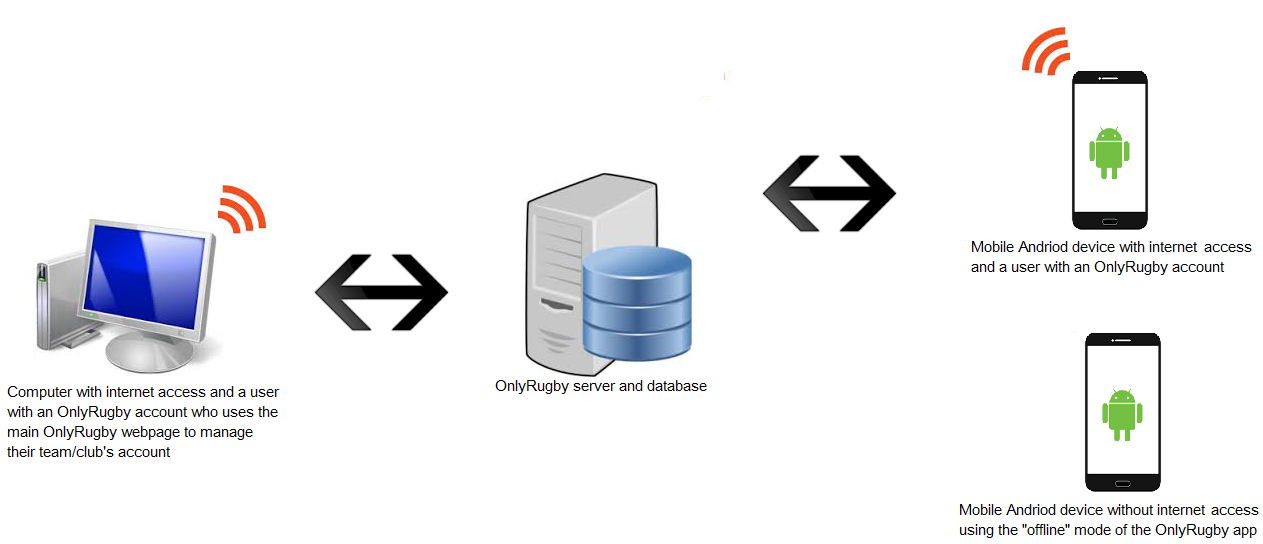
\includegraphics[width=0.9\textwidth] {./images/SystemConfiguration2.png}\\[0.4cm]
\end{center}
\section{Installation}
\begin {itemize}
	\item The user will have to choose to download the app from the Google App store (once released) and the rest will be done automatically by the app store itself. The user will be notified when the app is finished downloading and is ready to run. (Yet to be implemented).
	\item Alternativley the user could go on GitHub (https://github.com/hermankeuris/OnlyRugbyApp/tree/master/Instal)l and download the application's APK directly (i.e. Only Rugby Score Keeper.apk). You can either download this through your mobile device's web browser directly or first download it on a computer and then copy the APK file to your andriod device through a USB connection with the computer.
	\begin{center}
  		 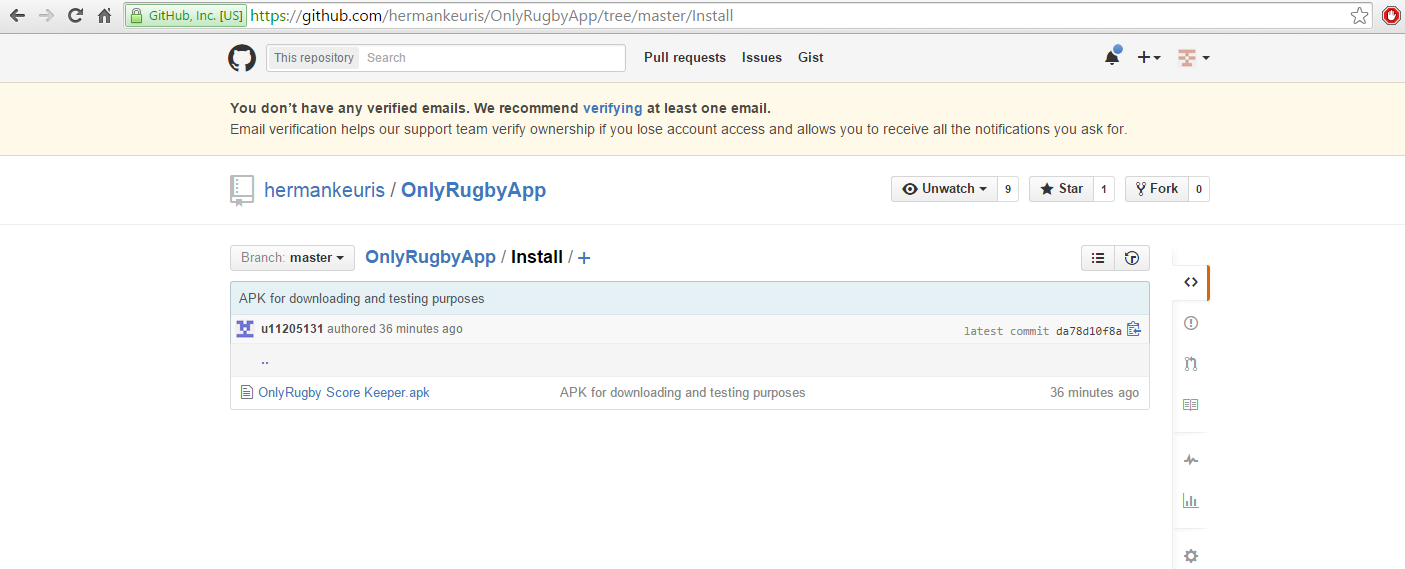
\includegraphics[width=0.9\textwidth] {./images/APKdownload.png}\\[0.4cm]
	\end{center}
	\item To allow your Andriod device to run this APK you will first have to enable your device to allow the installation of files from ''unknown'' sources. This is done by going to your device's Settings > Security and checking the ''Unknown Sources'' checkbox.
	\begin{center}
  		 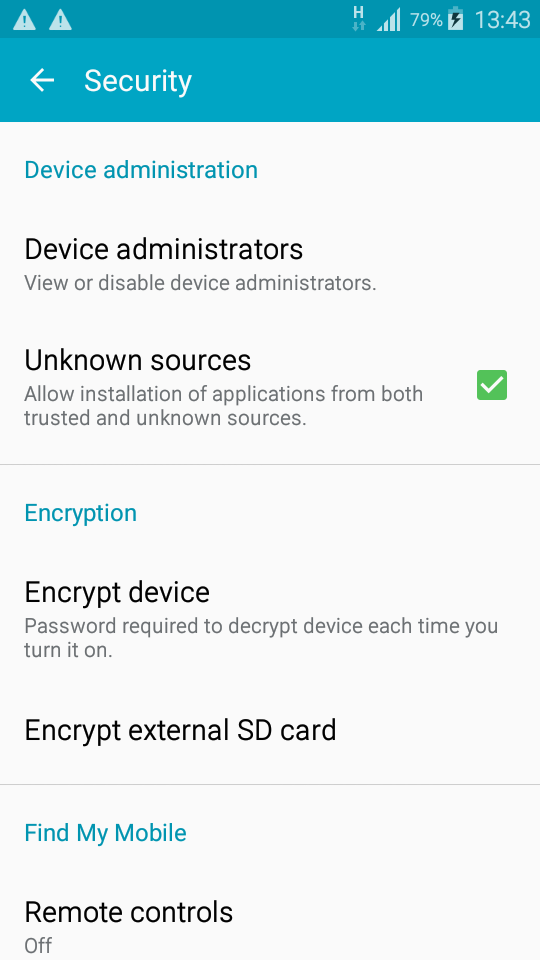
\includegraphics[width=0.3\textwidth] {./images/unknownsources.png}\\[0.4cm]
	\end{center}
	\item In the case of having directly downloaded the APK on your Android device you could then go to the directory where the APK is stored (most likely the ''Downloads'' folder) and click the APK's icon. A pop-up will then appear giving you the option of installing the APK on your device.
	\item In the case of having first downloaded the APK on a computer you should then copy the APK file to some easily accessible directory on the Android device (e.g. ''Downloads'') and then follow the same steps as specified in the previous bullet.
	\begin{center}
  		 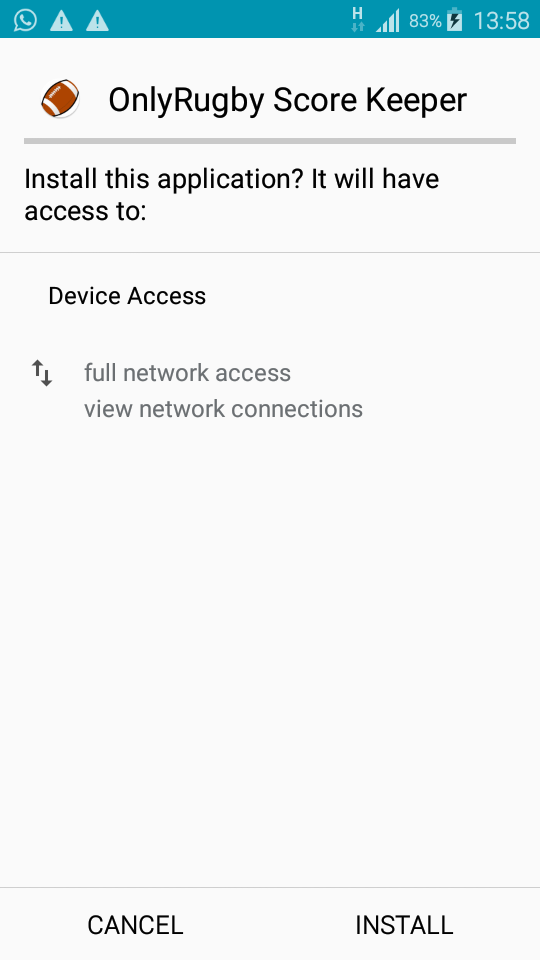
\includegraphics[width=0.3\textwidth] {./images/installation.png}\\[0.4cm]
	\end{center}
	\item To be able to use the application to its full potential the user will have to have both themselves and their club/team registered on the main OnlyRugby website. The user will also have to be registered as having the proper authority to log match information on behalf of his/her club/team. (Yet to be implemented).
	\item Note that for demo and testing purposes, all login and data upload functionality within the application have been temporarily disabled to increase ease of use.
\end{itemize}

\section{Getting started}
	\begin {itemize}
		\item To get access to use the app, the team you represent should already be registered with the main site.
		\item You also need to have a personal account and your team should have chosen you as their dedicated score keeper.
		\item When all the requirements are satisfied, simply log on to the app with your credentials as you registered them on the website.
		\item Once logged on, you can choose which match to score (pertaining only to your own team of course)
		\item You will not be permitted to score a match that is not in the progress of being played.
		\item Once a match is available to score, you can start the process by tapping on the relevant match and starting the procedure. From here you can log different states of the game, such as tackles, scores, line-outs, substitutions etc.
		\item Once a match is completed, the information can be verified or corrected as needed (such as adding unknown player's names) before being finally submitted to the server for storage in the main database.
		\item Usernames are unique and cannot be changed once you have registered it.
		\item Passwords can be changed using the websites Change Password function in account settings.
		\item Pressing the "back" button on your device twice pops up a notification asking if you really want to exit to prevent accidental app closure. Choosing "Yes" will close the app and all relevant main threads running.
	\end{itemize}
	
\newpage

\section{Using the system}
The functionality of the app will be spread between the following use cases:

	\subsection{Login/Logout}
		\begin {itemize}
			\item The first screen after choosing "Login" on the main screen, the user will be presented with two fields: One for the username and one for the password. The user enters the requested details and it gets authenticated. Only when the correct information is supplied, will the user be able to continue to the game menu.
			\item The login information will be used to load the next game that needs scoring.
			\item The user gets logged out of the app every time they exit, allowing someone else to be able to log in as well and ensuring security of information.
		\end{itemize}
		
  		\begin{minipage}[b]{0.4\textwidth}
    			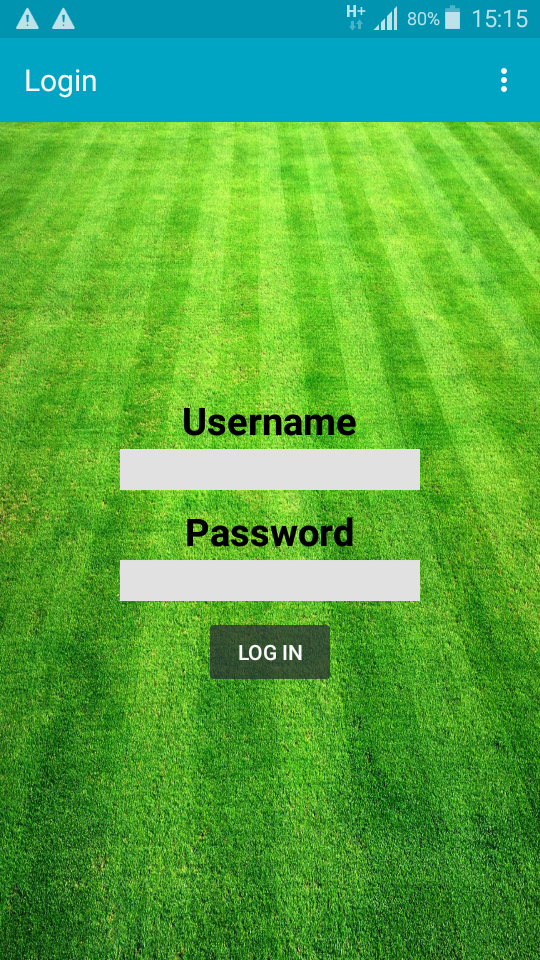
\includegraphics[width=0.9\textwidth]{./images/login_menu.png}
  		\end{minipage}

		
	\subsection{Load Info}
		This use case pertains to the loading of any and all info you can see and not see in the app itself. A version of it is called by nearly every other function in the app, since it handles all the retrieval from the database via the main server.
		\begin{itemize}
			\item After the user is logged in, information is loaded on what teams the user is allowed to score for and when their matches would take place. This is done by sending a query with the token (already received when logging in) to the server and retrieving the information associated with this particular user. All of the information is stored on the device's local database for offline usage.
			\item After selecting the appropriate team, the user can view the matches available / scheduled for that team.
			\item In the event that a match can be scored and the user decides to do so, the data pertaining to that match will be loaded from the device's local database, since it is already stored from the previous request to the server. This will return the names and positions of the players of both teams (if available).
			\item During the match, local storage is implemented to store any data relevant to the match and then uploaded once the app establishes a connection with the server.
		\end{itemize}

	\subsection{Game Time}
	This use case is used to log the start and end time of each half of a match, as well as any intervals during which time was lost (the game was paused) and a reason for this time loss (injury, substitution, match official consultation, replacement of damaged player clothing). 
	\\ \\
	Usage:
	\begin{itemize}
		\item The game time is displayed at the top of the UI.
		\item One starts the clock by tapping on it once. Preferably at kick-off. In the future the user will be presented with a confirm option in the form of a pop up which will not affect the running clock if accepted and reset the clock if denied.
		\item Once the clock is running a single tap on the clock will register a pause and activate a pop up asking the user for a reason for the pause, along with the legal options. The user will also have the option return should they accidentally activate this function. After a legal reason has been given for the pause the user is presented with a blank page and a button to resume the game.
		\item Upon reaching 40 minutes the game clock:
		\begin{itemize}
		\item registers the end of the current half,
		\item resets for the next half if there is one, and
		\item resets for overtime if conditions for it are met.
		\end{itemize}
	\end{itemize}

\newpage

	\subsection{Scoring}
		During game time (i.e. while the OnlyRugby app is being used to log the information of a match currently being played ) the Scoring function will be used each time a player from either team scores points for their team (be it through a try, penalty kick, drop-kick or a conversion kick following a try). The Scoring function works as follows:
		\begin{enumerate}
			\item At the main menu for the match logger the user gets to specify what type of score it should log. This page displays buttons titled 'Try', 'Penalty Kick' and  'Drop-kick' (note that 'Conversion Kick' is not an option as it can only be attempted after a successful try). 
		\begin{center}
	 	 	 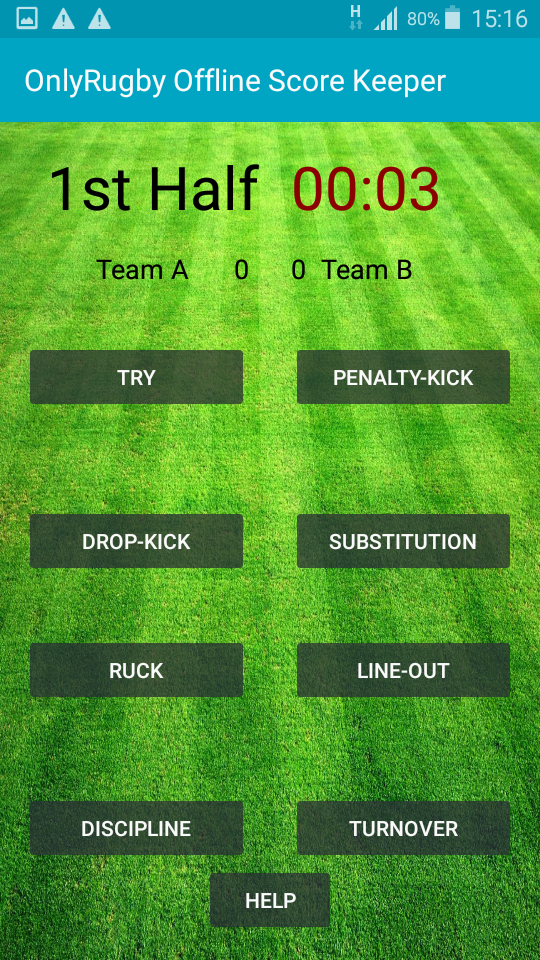
\includegraphics[width=0.3\textwidth] {./images/game_menu.png}\\[0.4cm]
		\end{center}
			\item Once the user has selected a score type and pressed the relevant  button to log that type's score information they are redirected to a page which asks them to indicate which team scored by pressing either of two buttons which each have the names of the respective teams on them.
		\begin{center}
  			 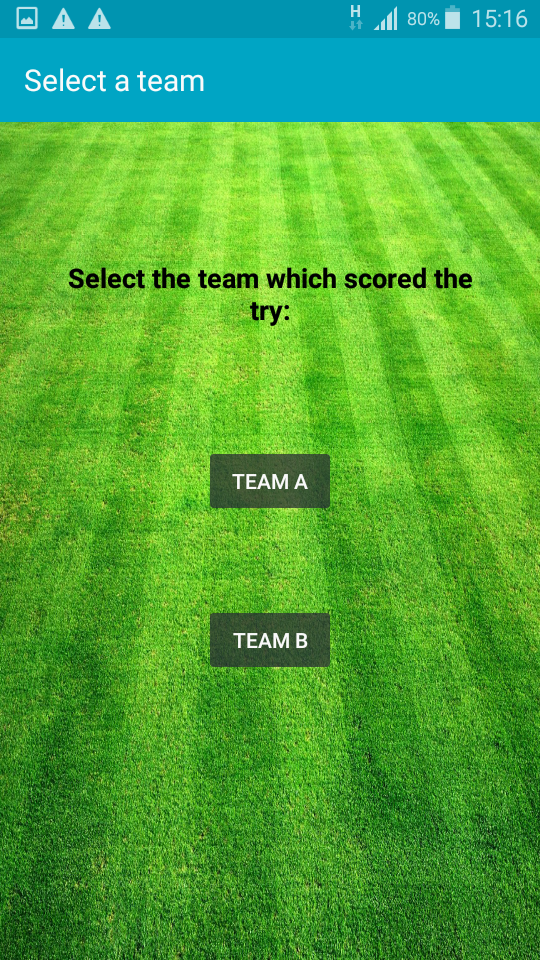
\includegraphics[width=0.3\textwidth] {./images/choose_try_team.png}\\[0.4cm]
		\end{center}
			\item The app then redirects the user to another page which has a list of 16 options representing the 15 on-field players of the previously selected team and an 'Unknown' option. Each option has the player's position/jersey number on it as well as the player's name (if that information is provided on the database). This 'Unknown' option is in case the user, for some reason, is not sure who scored on this team. The user is asked to select one of these players/buttons as the player who scored.
		\begin{center}
  			 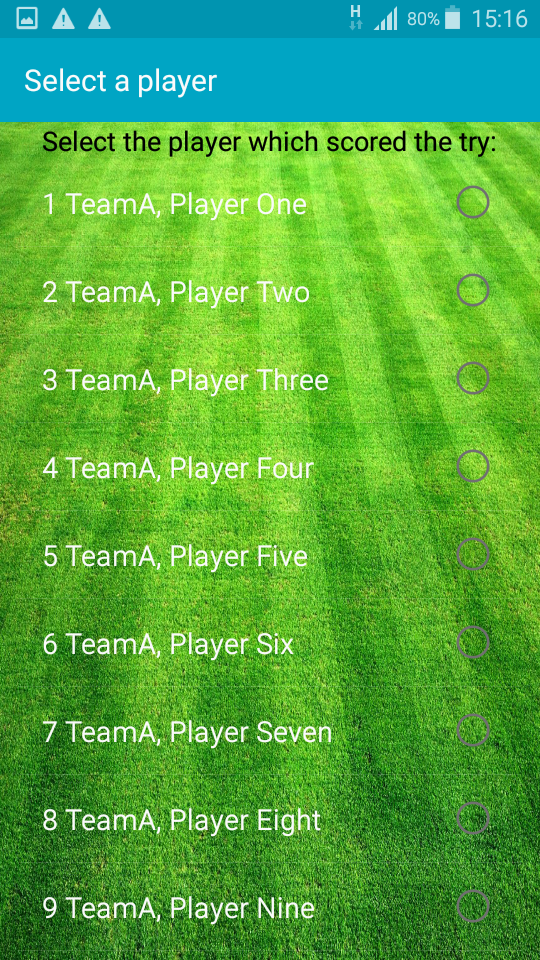
\includegraphics[width=0.3\textwidth] {./images/choose_try_player.png}\\[0.4cm]
		\end{center}
			\item In most cases the user is then done entering the score information but in the case of a 'Try' more steps must be completed:
				\begin{itemize}
					\item The user is first asked by a small pop-up message if the try was assisted by any other players with the options of clicking 'Yes' or 'No'. In the case of 'Yes' the user is then redirected to the same 'player selection page' as previously described were the user can then select a player which assisted the first player to score the try. (Note this function is not yet implemented as it is subject to change pending a meeting with the client).
					\item The player is then asked by another small pop-up message if the subsequent conversion kick was successful with the options of clicking 'Yes' or 'No'. Selecting 'Yes' once again redirects the user to the 'player selection page' to select a player which successfully scored the conversion kick.
				\begin{center}
  					 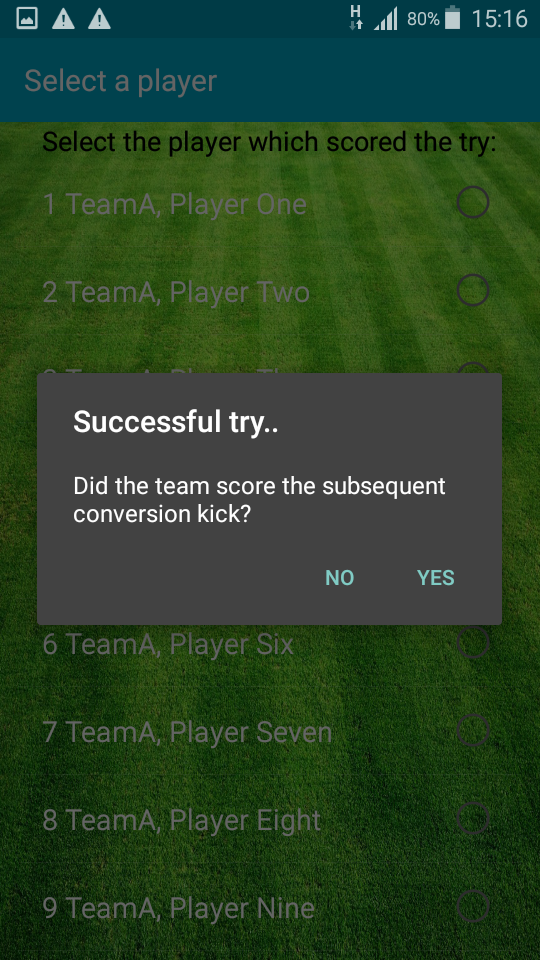
\includegraphics[width=0.3\textwidth] {./images/try_converted.png}\\[0.4cm]
				\end{center}
				\end{itemize}
		\item After a score has been logged the user is returned to the main match logger menu and the relevant team's score is updated.
		\begin{center}
  			 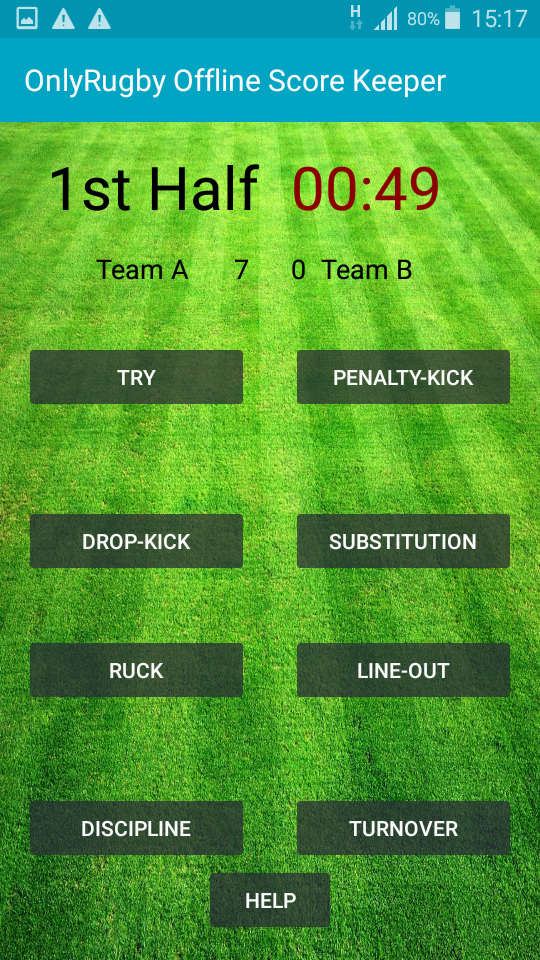
\includegraphics[width=0.3\textwidth] {./images/score_increased.png}\\[0.4cm]
		\end{center}
		\end{enumerate}
	On all of the above described pages the user also has the option of using the phone's  'Back' button which redirects the user to the previous page and ignores the information that was logged on the page it is now leaving.

	\subsection{Substitutions}
		During game time the Substitutions function will be used to log any changes made to both the on- and off-field players (i.e. reserve players) of either team. This function will work as follows:
		\begin{enumerate}
			\item Once the player has pressed the button to log player substitutions they are redirected to a page which asks them to indicate which team is substituting a player by pressing either of two buttons which each have the names of the respective teams on them.
			\begin{center}
  				 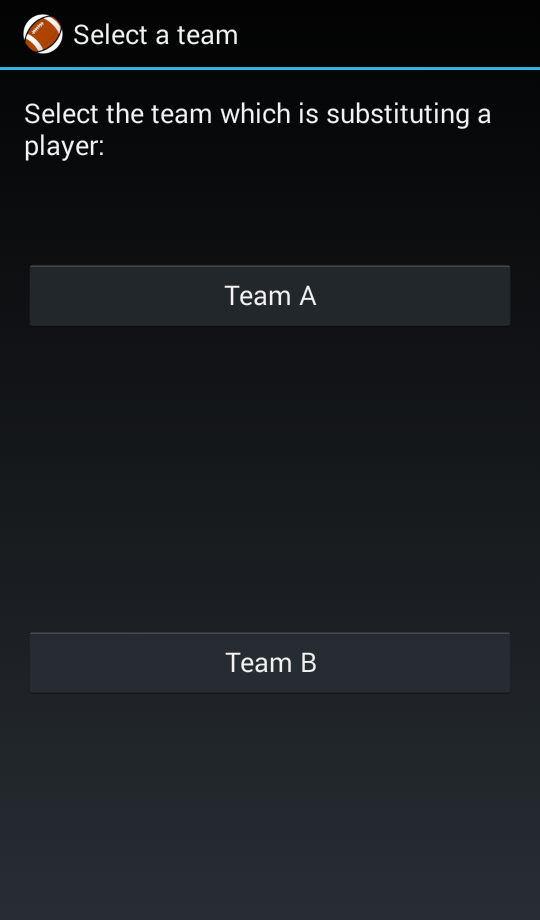
\includegraphics[width=0.3\textwidth] {./images/choose_substitute.png}\\[0.4cm]
			\end{center}
			\item The app then redirects the user to the 'player selection page' (as described in the Scoring section) which comprises of 15 options representing the on-field players of the selected team (i.e. without the 'Unknown' button). The user is then asked to select an on-field player which is being swapped out for a reserve player.
			\begin{center}
  				 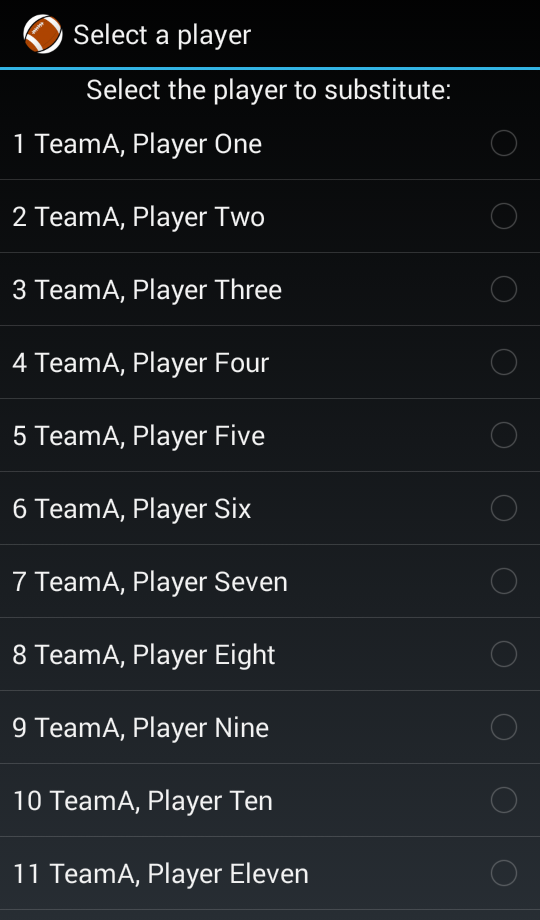
\includegraphics[width=0.3\textwidth] {./images/choose_substitute_player.png}\\[0.4cm]
			\end{center}
			\item The app then redirects the user to a page similar to the standard 'player selection page' which has between 0 and 7 options representing the reserve players of the selected team. These options also have the player's jersey numbers and names on them (if they are stored on the server's database). The user is then asked to select a reserve player to swap out with the previously selected on-field player. The two selected players then swap their places (i.e. the reserve is now on-field and vice versa). If there is not a full reserve team of 7 players stored on the server's database then the remaining players required to form a team of 7 are substituted with distinct 'Unknown' players to hold place for any players which might function as reserve players during match time but who were not logged on the main site's database (which means the app therefore does not have information about them).
	On all of the above described pages the user also has the option of using the phone's  'Back' button which redirects the user to the previous page and ignores the information that was logged on the page it is now leaving.
		\begin{center}
  				 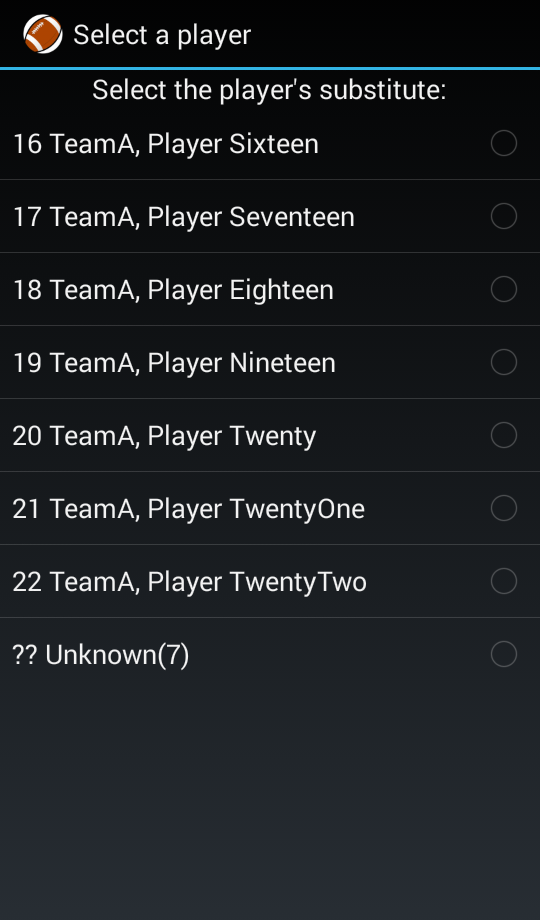
\includegraphics[width=0.3\textwidth] {./images/choose_substitute_off_field.png}\\[0.4cm]
			\end{center}
		\end{enumerate}
	\subsection{Discipline}
		During game time (i.e. while the OnlyRugby app is being used to log the information of a match currently being played ) the Discipline function will be used each time a player performs an infraction that causes them to receive a card. The Discipline function works as follows:
		\begin{enumerate}
			\item Once the user has pressed the button to log the disciplinary action's information they are redirected to a page which asks them to indicate which team's player was given a card, by pressing either of two buttons which each have the names of the respective teams on them.
			\item The app then redirects the user to another page which has 15 buttons representing the 15 on-field players of the previously selected team. Each button has the player's position/jersey number on it as well as the player's name (if that information is provided on the database). This page also has an 'Unknown' button in case the user, for some reason, is not sure who the player being disciplined is. The user is asked to select one of these players/buttons as the player who was disciplined.
			\item The app then redirects the user to another page which has 3 buttons, to indicate if a white, yellow or red card was given.
		\end{enumerate}
	On all of the above described pages there are also buttons labelled 'Cancel' (to cancel logging the discipline) and 'Back' which redirects the user to the previous page and ignores the information that was logged on the page it is now leaving.

	\subsection{Line-outs}
	During game time the Line-outs function will be used to log when the ball has gone out of the field of play and a line-out has occurred. The team that manages to take possession of the ball during the line-out is the winner. This function will work as follows:
	\begin{itemize}
		\item Once the user has pressed the button to log the line-out's information they are redirected to a page which asks them to indicate which team won the line-out by pressing either of two buttons which each have the names of the respective teams on them.
	\end{itemize}
	On the above described page there is also a button labelled 'Cancel' (to cancel logging the line-out) and 'Back' which redirects the user to the previous page and ignores the information that was logged on the page it is now leaving.

	\subsection{Scrums}
	{\bfseries\{This section is still under development\}}
		\begin{itemize}
			\item The scrum button will be on the game page when a game scoring is in progress.
			\item It will then ask who won the scrum.
		\end{itemize}
		
	\subsection{Tackles}
	{\bfseries\{This section is still under development\}}
		\begin{itemize}
			\item During a match, the user will have the option to log if and when a tackle was performed (the "when" is logged by using a time stamp value).
			\item Tapping on tackle will provide the user with the means of choosing who performed the tackle, as well as if the tackle was successful or not.
		\end{itemize}

	\subsection{Possession \& Turnovers}
		At the start of the match the player must indicate which of the two teams initially gains possession of the ball by clicking one of two buttons which have the names of the two teams on them. After that the player can easily indicate a change in possession by pressing a small button on the main tool bar which can be seen on each page.
		\\
		During game time (i.e. while the OnlyRugby app is being used to log the information of a match currently being played ) the Turnover function will be used each time a player from either team manages to take possession of the ball from an opposing player. The Turnover function works as follows:
		\begin{enumerate}
			\item Once the user has pressed the button to log the turnover's information they are redirected to a page which asks them to indicate which team won the turnover by pressing either of two buttons which each
			have the names of the respective teams on them.
			\item The app then redirects the user to another page which has 15 buttons representing the 15 on-field players of the previously selected team. Each button has the player's position/jersey number on it 
			as well as the player's name (if that information is provided on the database). This page also has an 'Unknown' button in case the user, for some reason, is not sure who won the turnover. The user is asked to select one of these players/buttons as the player who won the turnover.
			\item The user is then redirected to a page, similar to the one above, that has a list of the other team's 15 on-field players. Here, the user selects the player who lost the ruck.
		\end{enumerate}
	On all of the above described pages there are also buttons labelled 'Cancel' (to cancel logging the turnover) and 'Back' which redirects the user to the previous page and ignores the information that was logged on the page it is now leaving.


		\begin{figure}[!htb]
  		\centering
  			\begin{minipage}[b]{0.4\textwidth}
    			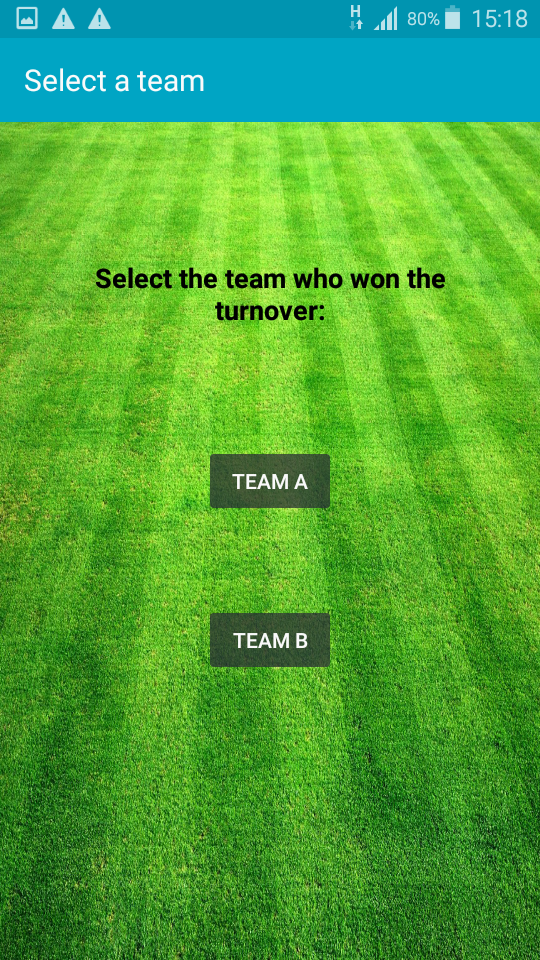
\includegraphics[width=0.9\textwidth]{./images/choose_turnover.png}
    			\caption{Choose team who won the turnover}
  			\end{minipage}
  		\hfill
		\end{figure}

	\subsection{Clean break}
	{\bfseries\{This section is still under development\}}
		\begin{itemize}
			\item The clean break button will be on the game page when a game scoring is in progress.
			\item It will then ask the player that performed the clean break.
		\end{itemize}

	\subsection{Offloads}
	{\bfseries\{This section is still under development\}}\\ \\
	Currently not implemented. Usage likely to be similar to the following description:
	\begin{itemize}
		\item Offload button present on landing page after login.
		\item Button can only be activated during game time.
		\item Activating the button registers an offload and presents a pop up prompt asking for:
			\begin{enumerate}
				\item The team to which the offload was given. (2 buttons)
				\item The player that performed the offload, by player number or by name. (Defaults to "unknown player").
			\end{enumerate}
		\item An option to cancel the offload will also be present along with return option
		\item Activating the return button will prompt the user to save data as default, what the user entered, or to cancel the registering of an offload.
	\end{itemize}
	\subsection{Ruck}
		During game time (i.e. while the OnlyRugby app is being used to log the information of a match currently being played ) the Ruck function will be used each time the ball is on the ground and players are crowded around it.During this time, they must use their feet to manoeuvre it to the back of the rear player's feet, at which point it may be picked up. The Ruck function works as follows:
		\begin{enumerate}
			\item Once the user has pressed the button to log the ruck's information they are redirected to a page which asks them to indicate which
			team won the ruck by pressing either of two buttons which each have the names of the respective teams on them.
		\end{enumerate}
		\begin{center}
  			 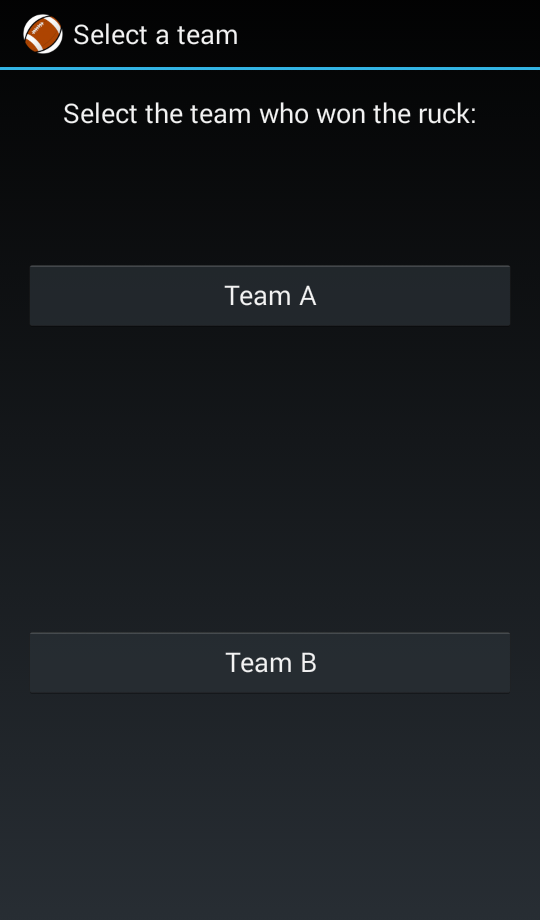
\includegraphics[width=0.3\textwidth] {./images/choose_ruck_team.png}\\[0.4cm]
		\end{center}
	On all of the above described pages the user also has the option of using the phone's  'Back' button which redirects the user to the previous page and ignores the information that was logged on the page it is now leaving.

	\subsection{Maul}
	{\bfseries\{This section is still under development\}}
		\begin{itemize}
			\item When scoring a match, the user will have the option to log when a maul occurs.
			\item The team who has possession will be logged, as well as the specific player, if at all possible.
		\end{itemize}

\section{Troubleshooting}
	{\bfseries\{This section is still under development\}}\\ \\
	In the event that the app crashes or something goes wrong, a comprehensive error message will be provided to the user with an error code. This error code can then be used with the built-in troubleshooting guide for a more descriptive explanation of the error. Additionally, an error log file will also be created, containing all the relevant information pertaining to the crash.
		
\end{document}
